\documentclass[15pt]{beamer}
\title{LUDO}
\date{27th March 2021}
\author[Bvrith]{K.Sai Amulya : 19WH1A0446 : ECE \\ Ch.Sowmya : 19WH1A05G9 : CSE \\ N.Tushara : 19WH1A0519 : CSE \\ P.Siri Hasitha : 19WH1A1293 : IT \\ M.Shravani : 19WH1A0407 : ECE}
\usefonttheme{serif}
\usepackage{bookman}
\usepackage{hyperref}
\usepackage[T1]{fontenc}
\usepackage{graphicx}
\usecolortheme{orchid}
\beamertemplateballitem
\graphicspath{./images/}


\begin{document}
    \begin{frame}
        \titlepage
	    \begin{center}
	 BVRIT HYDERABAD College of \\ Engineering for Women
	    \end{center}
    \end{frame}

    \begin{frame}
    \frametitle{Introduction}
        \begin{figure}

		\begin{center}
		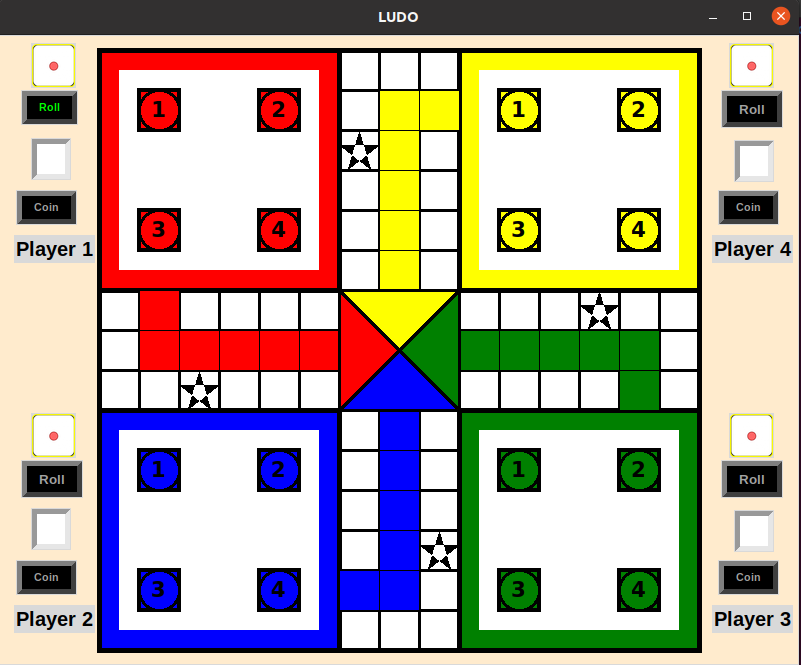
\includegraphics[width=0.9\linewidth]{board_1.png}
		\end{center}
        \end{figure} 
    
    \end{frame}

  
    \begin{frame}
	    \frametitle{Approach}
	    \begin{itemize}
		    \item Bring the coins to start position after rolling a die
	            \item Coin movement
	            \item Repeat chance
		    \item Coin overlap
		    \item Homepath traversal and coin reaching home
		    \item Check for winner and runner
	    \end{itemize}
    \end{frame}

    \begin{frame}
	    \frametitle{Learnings}
	    	\begin{itemize}
			\item Version control - git
			\item LaTeX
			\item Pygame
			\item Tkinter
			\item Pillow
			\item OOP
			\item Multimedia in Tkinter and Pygame
		\end{itemize}
    \end{frame}

    \begin{frame}
	    \frametitle{Challenges}
	    \begin {itemize}
    	
		\item Unable to divide the gameboard into equal parts
		\item Coloring the homepath with smaller rectangles
		\item Player coin code not suitable for coin movement
			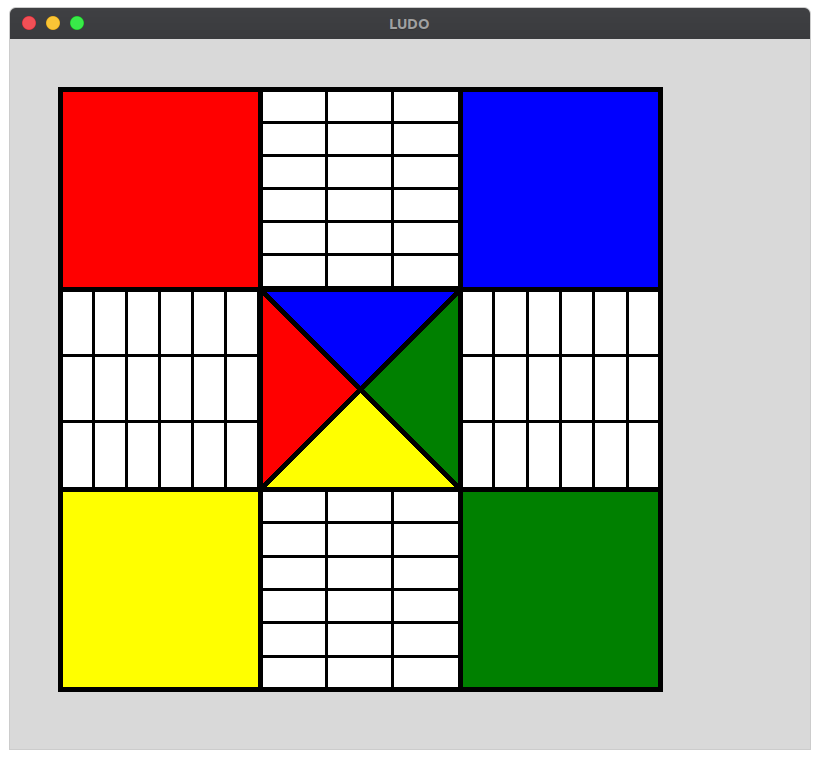
\includegraphics[width=0.35\linewidth]{stage4.png}
        	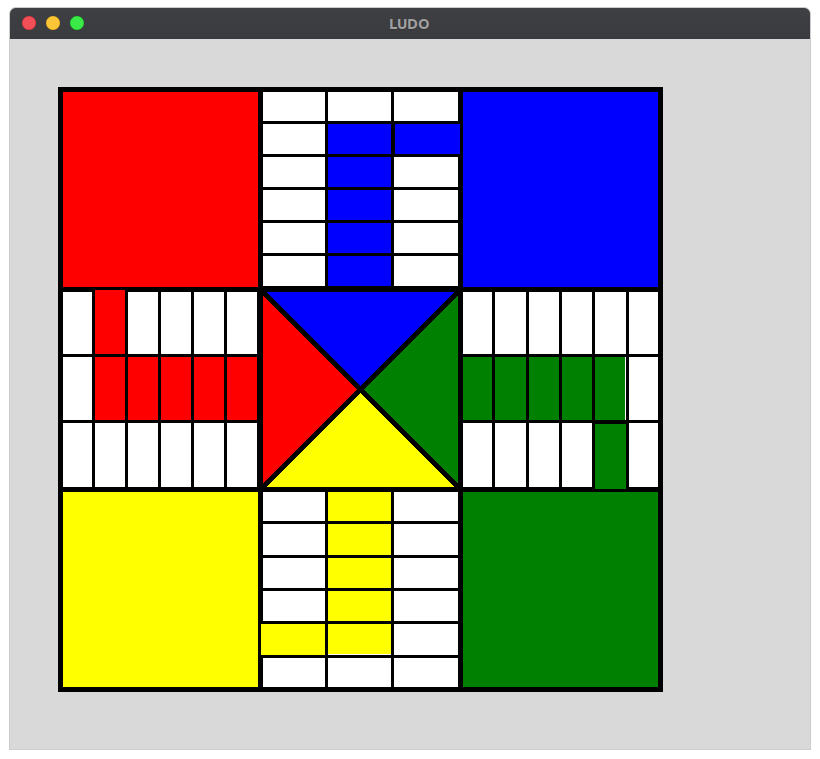
\includegraphics[width=0.35\linewidth]{stage5.png}
		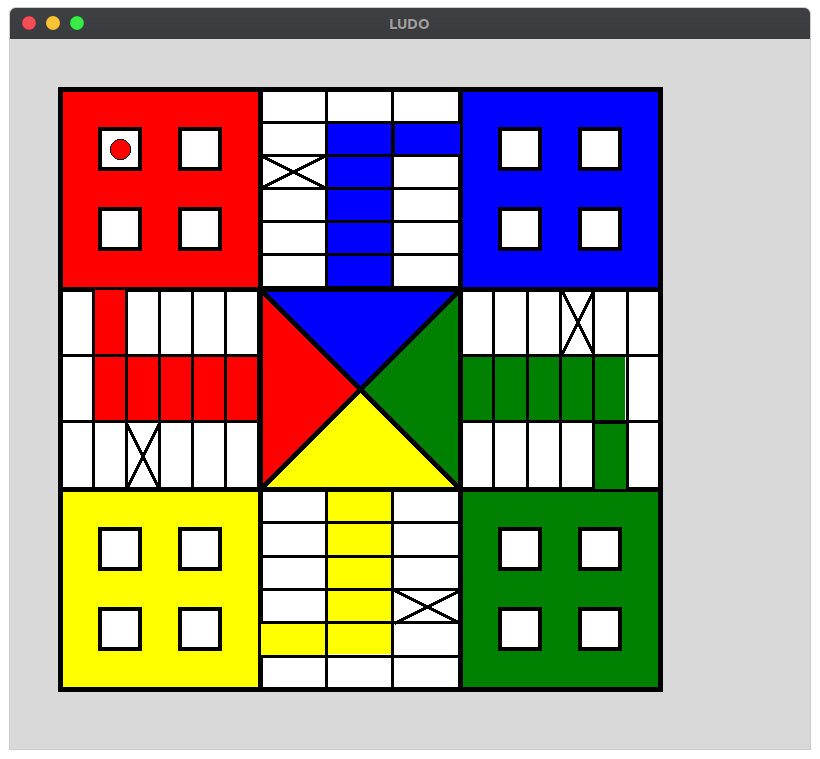
\includegraphics[width=0.35\linewidth]{stage6.png}
		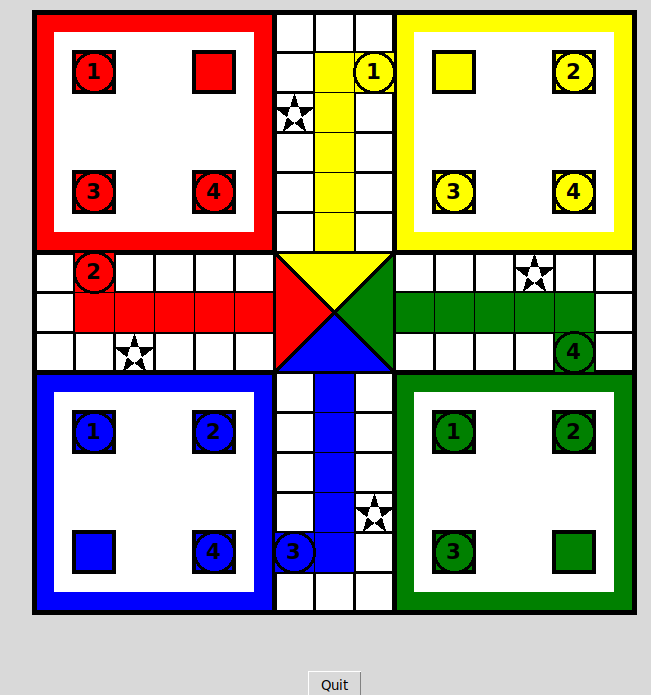
\includegraphics[width=0.35\linewidth]{board_with_start_positions.png}
		

	    \end{itemize}
    \end{frame}

    \begin{frame}
	    \frametitle{Challenges}
	    \begin{itemize}
	      
              \item Rolling dice and images as buttons
	      \item Unable to test each part of the code individually
		\end{itemize}

		      \begin{figure}
		      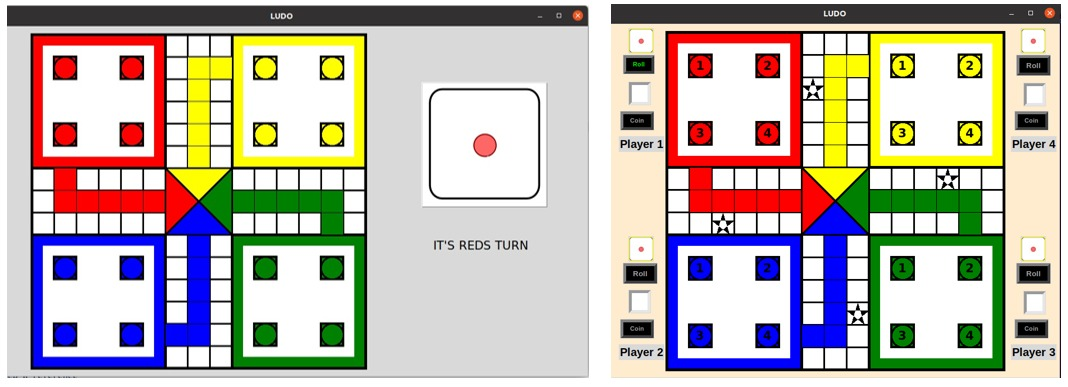
\includegraphics[width=1\linewidth]{dice.jpeg}
                          
		      \end{figure}
		
    \end{frame}

    
	
        


    \begin{frame}
    \frametitle{GIT Repo}
    \begin{figure}
	    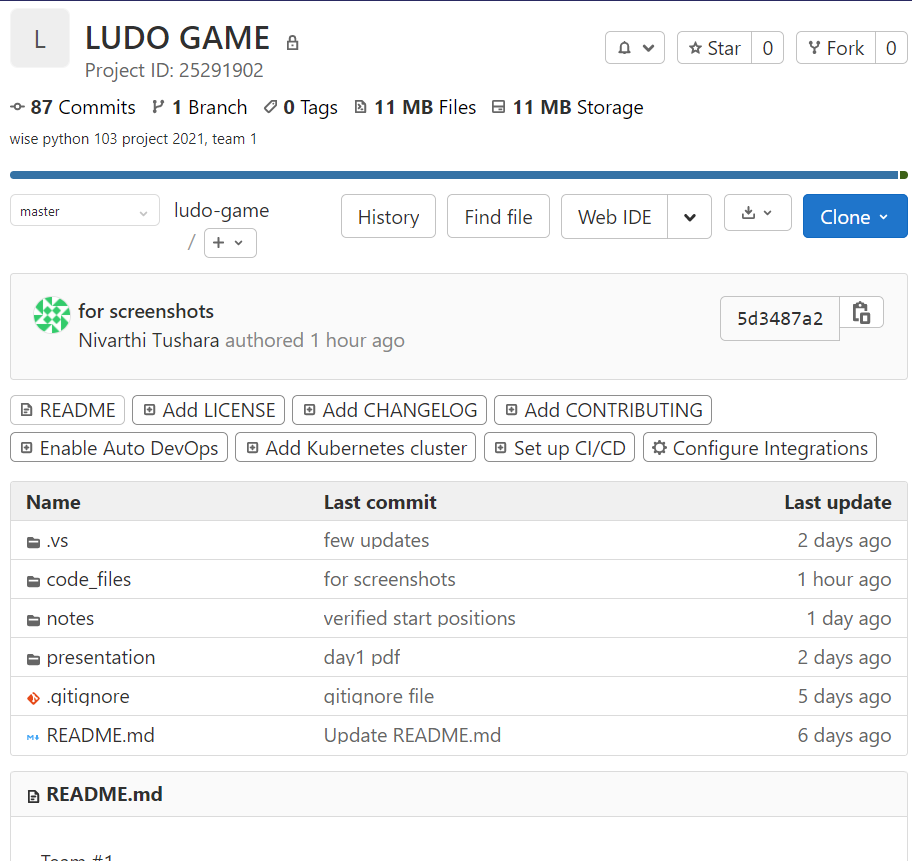
\includegraphics[width=0.9\linewidth]{final_repo.png}
	    
    \end{figure}
    \end{frame}

    \begin{frame}
    \frametitle{Statistics}
        \begin{itemize}
         \item Number of Lines of Code : 1247
         \item Number of Functions : 25
	 \item Number of Libraries : 5 
        \end{itemize}
    \end{frame}
    \begin{frame}
	    \begin{center}
		    LET'S PLAY THE GAME!
	    \end{center}
    \end{frame}
        


    \begin{frame}
	    \frametitle{Bibliography}
	    	\begin{itemize}
			\item https://docs.python.org/3/library/tk.html
			\item https://www.youtube.com/watch?v=edureka
			\item https://www.youtube.com/watch?v=cJbnWZGX-XY\&t=51s\&abchannel=edureka
			\item https://www.pygame.org/docs/
		 
		\end{itemize}
    \end{frame}
    \begin{frame}
	    \frametitle{Meet the team!}
	    \begin{figure}
		    
\includegraphics[width=0.2\linewidth]{shravani.jpeg}
		    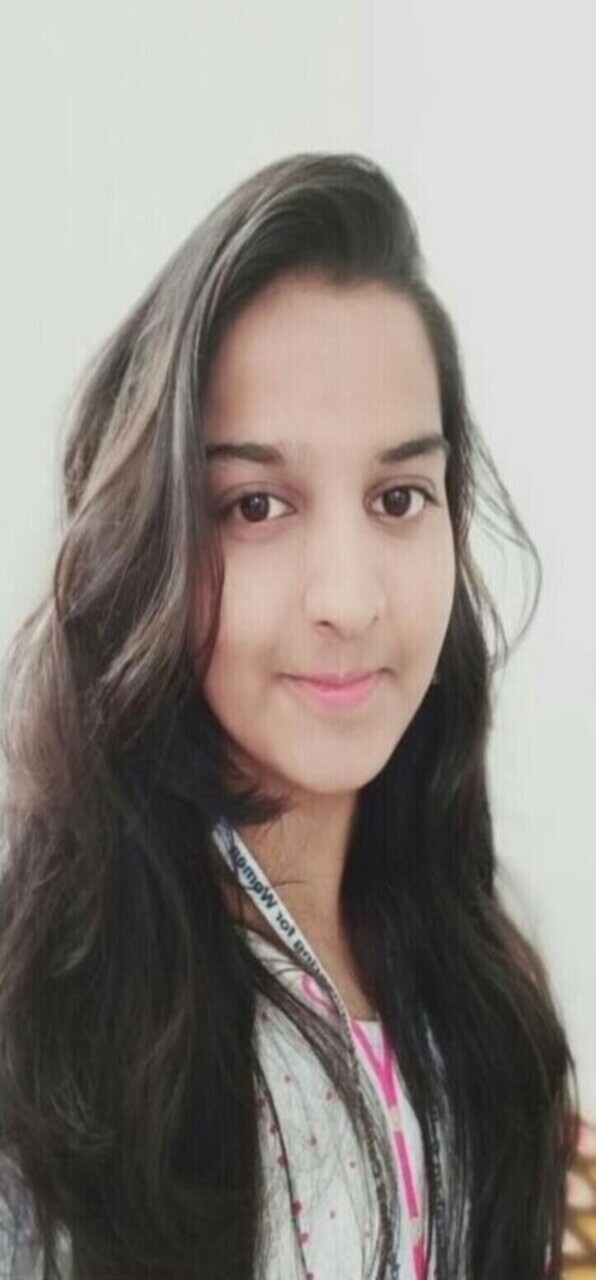
\includegraphics[width=0.2\linewidth]{siri.jpeg}
		    
\includegraphics[width=0.2\linewidth]{amulya.jpeg}
		    
\includegraphics[width=0.2\linewidth]{tushara.jpeg}
		    \end{figure}
    \end{frame}

    \begin{frame}
    \begin{center}
         THANK YOU
    \end{center}
    \end{frame}
\end{document}

